\section{Interlude: the arrow of time}

On a higher-level, one can view the Floquetification of the last section as a reinterpretation of the time direction
in a ZX-diagram.
Below, we use two blue prisms (square and hexagonal)
as abstractions of ZX-diagrams for the $\qcode{4, 2, 2}$ code and double hexagon code respectively.
In grey we show how a timeslice in the double hexagon code corresponds to an angled slice of the $\qcode{4, 2, 2}$ code:
\begin{equation}\label{eq:timeslice_4_2_2_double_hexagon}
\begin{aligned}
    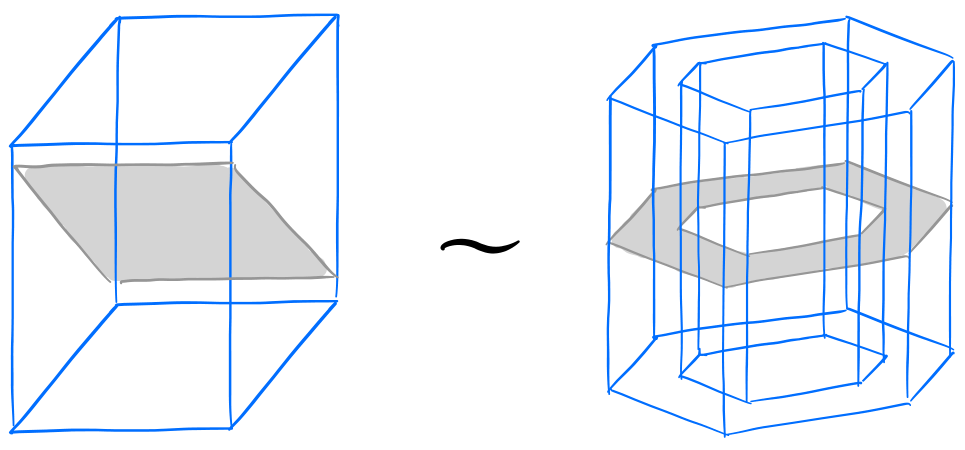
\includegraphics[width=230pt]{figures/qubits/floquetifying/422/floquetified/abstract_timeslice}
\end{aligned}
\end{equation}